\documentclass[10pt, letterpaper]{article}

\usepackage{cvpr}
\usepackage{times}
\usepackage{epsfig}
\usepackage{graphicx}
\usepackage{amsmath}
\usepackage{amssymb}

% Include other packages here, before hyperref.
\usepackage{bm}
% Include other packages here, before hyperref.
% zizhao package
\usepackage{tabularx} % in the preamble
\newcolumntype{Y}{>{\centering\arraybackslash}X}
\newcommand\VRule[1][\arrayrulewidth]{\vrule width #1}
\usepackage{array,booktabs,arydshln,xcolor} % for widening table line
\usepackage{amsthm}
\usepackage{epstopdf}
\usepackage{algorithm}
%\usepackage{algorithmic}
\usepackage{amsthm}
\usepackage{multirow}
\usepackage{multicol}
\usepackage[algo2e]{algorithm2e}
\usepackage[toc,page]{appendix}
\usepackage{blindtext}
% If you comment hyperref and then uncomment it, you should delete
% egpaper.aux before re-running latex.  (Or just hit 'q' on the first latex
% run, let it finish, and you should be clear).
\usepackage[breaklinks=true,bookmarks=false]{hyperref}

%\cvprfinalcopy % *** Uncomment this line for the final submission

\def\cvprPaperID{2823} % *** Enter the CVPR Paper ID here
\def\httilde{\mbox{\tt\raisebox{-.5ex}{\symbol{126}}}}

% Pages are numbered in submission mode, and unnumbered in camera-ready
%\ifcvprfinal\pagestyle{empty}\fi

\setcounter{page}{1}
\begin{document}
%\tableofcontents
%\blinddocument

%%%%%%%%% TITLE
%\title{Supplementary Materials for "Understanding, Describing, and Visualizing Medical Images Through Reading Diagnostic Report Text"}
\title{Supplementary material for Photographic Text-to-Image Synthesis \\ with a Hierarchically-nested Adversarial Network}
%\author{First Author\\
%Institution1\\
%Institution1 address\\
%{\tt\small firstauthor@i1.org}
%% For a paper whose authors are all at the same institution,
%% omit the following lines up until the closing ``}''.
%% Additional authors and addresses can be added with ``\and'',
%% just like the second author.
%% To save space, use either the email address or home page, not both
%\and
%Second Author\\
%Institution2\\
%First line of institution2 address\\
%{\tt\small secondauthor@i2.org}
%}

\maketitle
%\thispagestyle{empty}

%appendicesappendices%%%%%%%% ABSTRACT
%\begin{abstract}
%   The ABSTRACT is to be in fully-justified italicized text, at the top
%   of the left-hand column, below the author and affiliation
%   information. Use the word ``Abstract'' as the title, in 12-point
%   Times, boldface type, centered relative to the column, initially
%   capitalized. The abstract is to be in 10-point, single-spaced type.
%   Leave two blank lines after the Abstract, then begin the main text.
%   Look at previous CVPR abstracts to get a feel for style and length.
%\end{abstract}

%%%%%%%%% BODY TEXT


\section{Training and Architecture Details}
%The algorithm that summarizes the training process of our model is given in Algorithm 1. 
%We train and evaluate our model with a devbox machine. $\alpha$ is set to 0.5, $\beta$ is set to 4.
The training is similar to the standard alternative training strategy in GANs, which alternatively updates the generator and discriminators.
The Adam optimizer \cite{kingma2014adam} is used.  The initial learning rate is set as 0.0002 and decreased by half for every 100 epochs (50 for COCO). The model is trained for 500 epochs in total (200 epochs for COCO).
We configure  the side outputs at 4 different scales where the feature map resolution is equal to $64^2,128^2,256^2$, and $512^2$, respectively.
For the local image loss of these 4 side outputs, we set $R_1=1, R_2=1, R_3=5, R_4=5$. For example, $R_1$ refers to $64^2$. These numbers are not fine-tuned but are set empirically. We believe there exists better configurations.

All intermediate conv layers except from the specified ones in Section 3.4 use $3{\times}3$ kernels (with reflection padding).
Some other normalization layers are experimented (i.e. instance normalization \cite{ulyanov2016instance} and layer normalization \cite{ba2016layer}) since they are used by recent advances \cite{zhu2017unpaired,chen2017photographic}. But they are not satisfactory. 

With respect to the generator, we use 1-repeat residual blocks for the generator till the $256^2$ resolution. The input of the generator is a $1024{\times}4{\times}4$ tensor. As the feature map resolution increases by 2, the number of feature maps is downsampled also by $2$, at $8, 32, 128, 256$ sizes. 
To generate $512^2$ images, we pre-train the generator to $256^2$ due to the limitation of the GPU memory. We use a $3$-repeat res-block followed by a stretching layer to upscale the feature map size to $32{\times}512{\times}512$. and a linear compression layer to generate images. 
Since the $256^2$ image already captures the overall semantics and details, to encourage the $512^2$ maintain these information, we use a l1 reconstruction loss to `self-regularize' the generator in case the discriminator confuses the expected output.

All source code will be released for better understanding.

\section{More Qualitative Results and Analysis}
In this section, we demonstrate more sample results for the three datasets.

Figure \ref{fig:bird2} compares our results with StackGAN. For each input, 6 images are randomly sampled. The results demonstrate better visual quality than StackGAN.
Figure \ref{fig:bird} shows the results on the CUB bird dataset. All the outputs of a model with different resolutions are also shown. As can be observed in the two figures, our method can generate fairly vivid images with different poses, shape, background, etc. Moreover, the images with different resolutions, which are side outputs of a single model, have very consistent information. More and more image details can be observed as the resolution increases.
Figure \ref{fig:flower} shows the results on the Oxford-102 flower dataset. Very detailed petals can be generated with photographic colors and saturability.

Figure \ref{fig:coco} shows the examples on the COCO dataset. COCO is much more challenging than the other two datasets since it contains natural images from very different scenes containing hundreds of different objects. 
As can be observed in the shown samples, our method generate semantically consistent and meaningful images, which correctly interpret the input text. 

However, it is worth to notice that, although our method significantly improves existing methods \cite{han2017stackgan,reed2016generative} on COCO, we realize that generating fine-grained details of natural scenes is still challenging. The  generation of the real natural image domain remains unsolved. We expect to address this problem as the future study. 



\newpage


%\renewcommand{\thechapter}{A\arabic{chapter}}
%\subsection{Results on the CUB bird dataset}
\begin{figure}[th!]
	\centering
	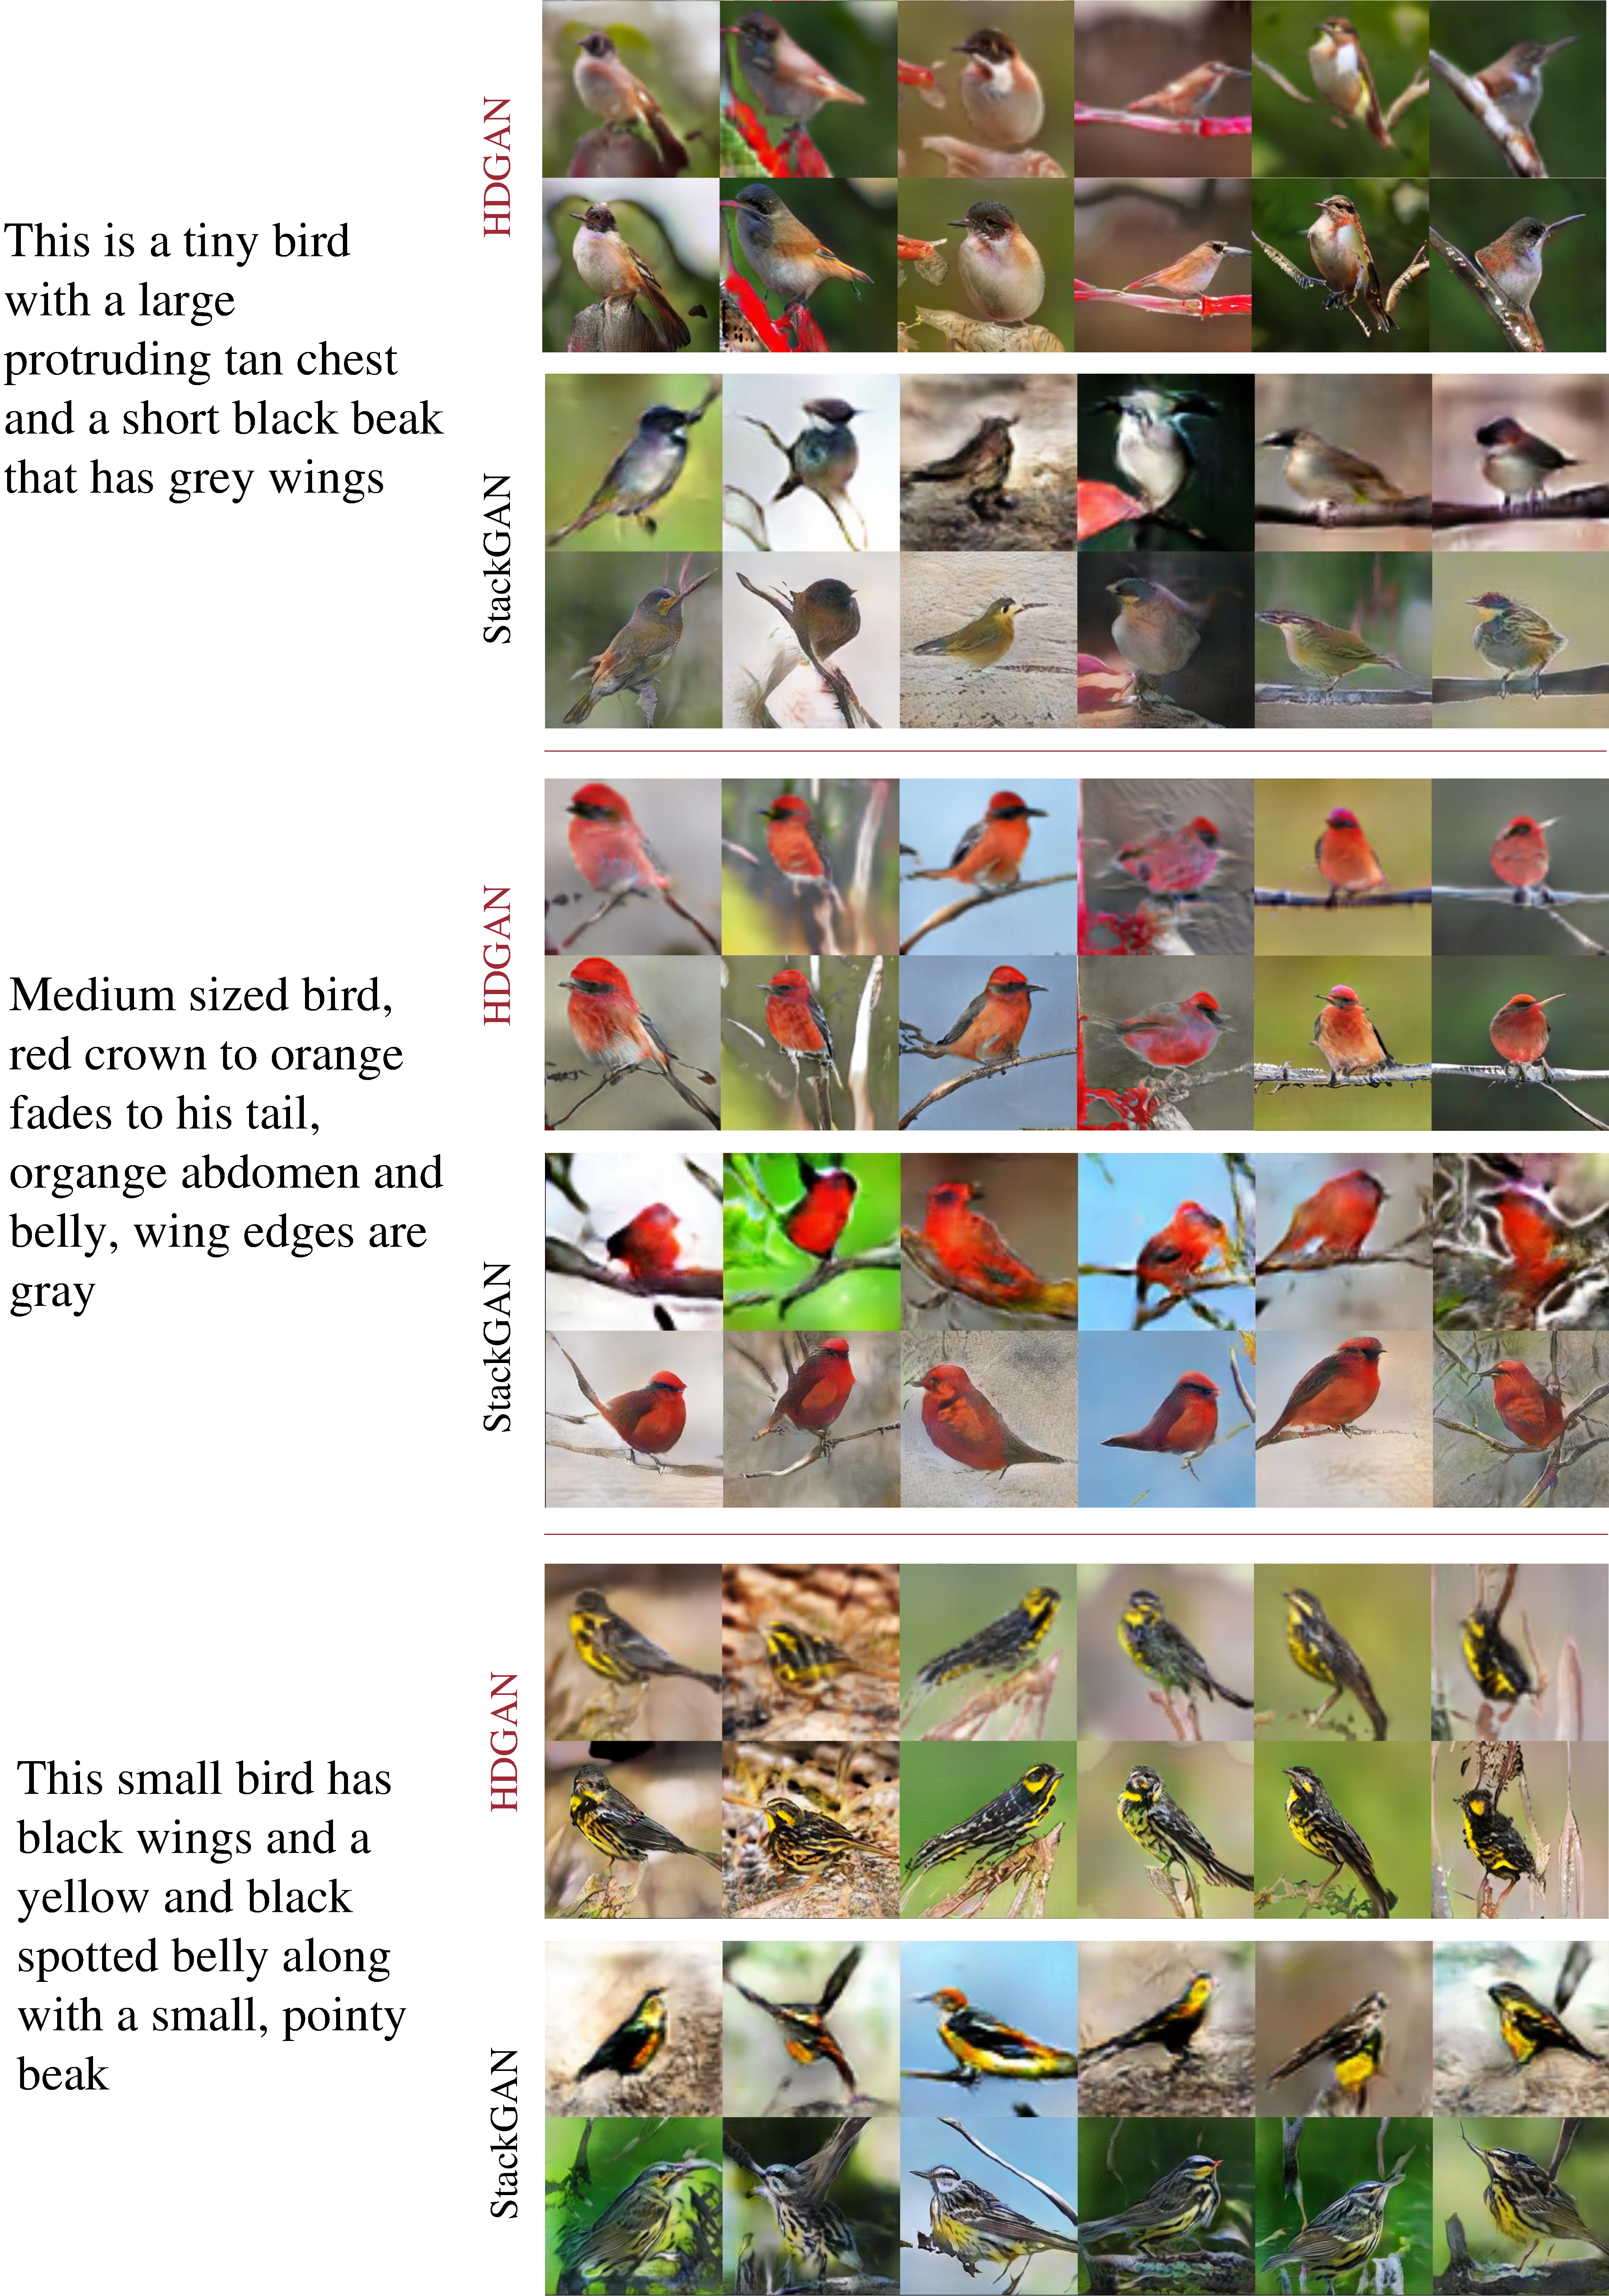
\includegraphics[width=0.83\textwidth]{figure/supp_bird2.pdf}
	
	\caption{Sample results on CUB compared with StackGAN. For each input, 6 samples are shown with resolutions of $64^2$ and $256^2$, respectively. As can be obviously seen, our HDGAN can generate very consistent content in images of different resolutions. Moreover, our generated images show more photographic color and contrast.  }  
	\label{fig:bird2}
\end{figure}
\newpage
\begin{figure}[th!]
	\centering
	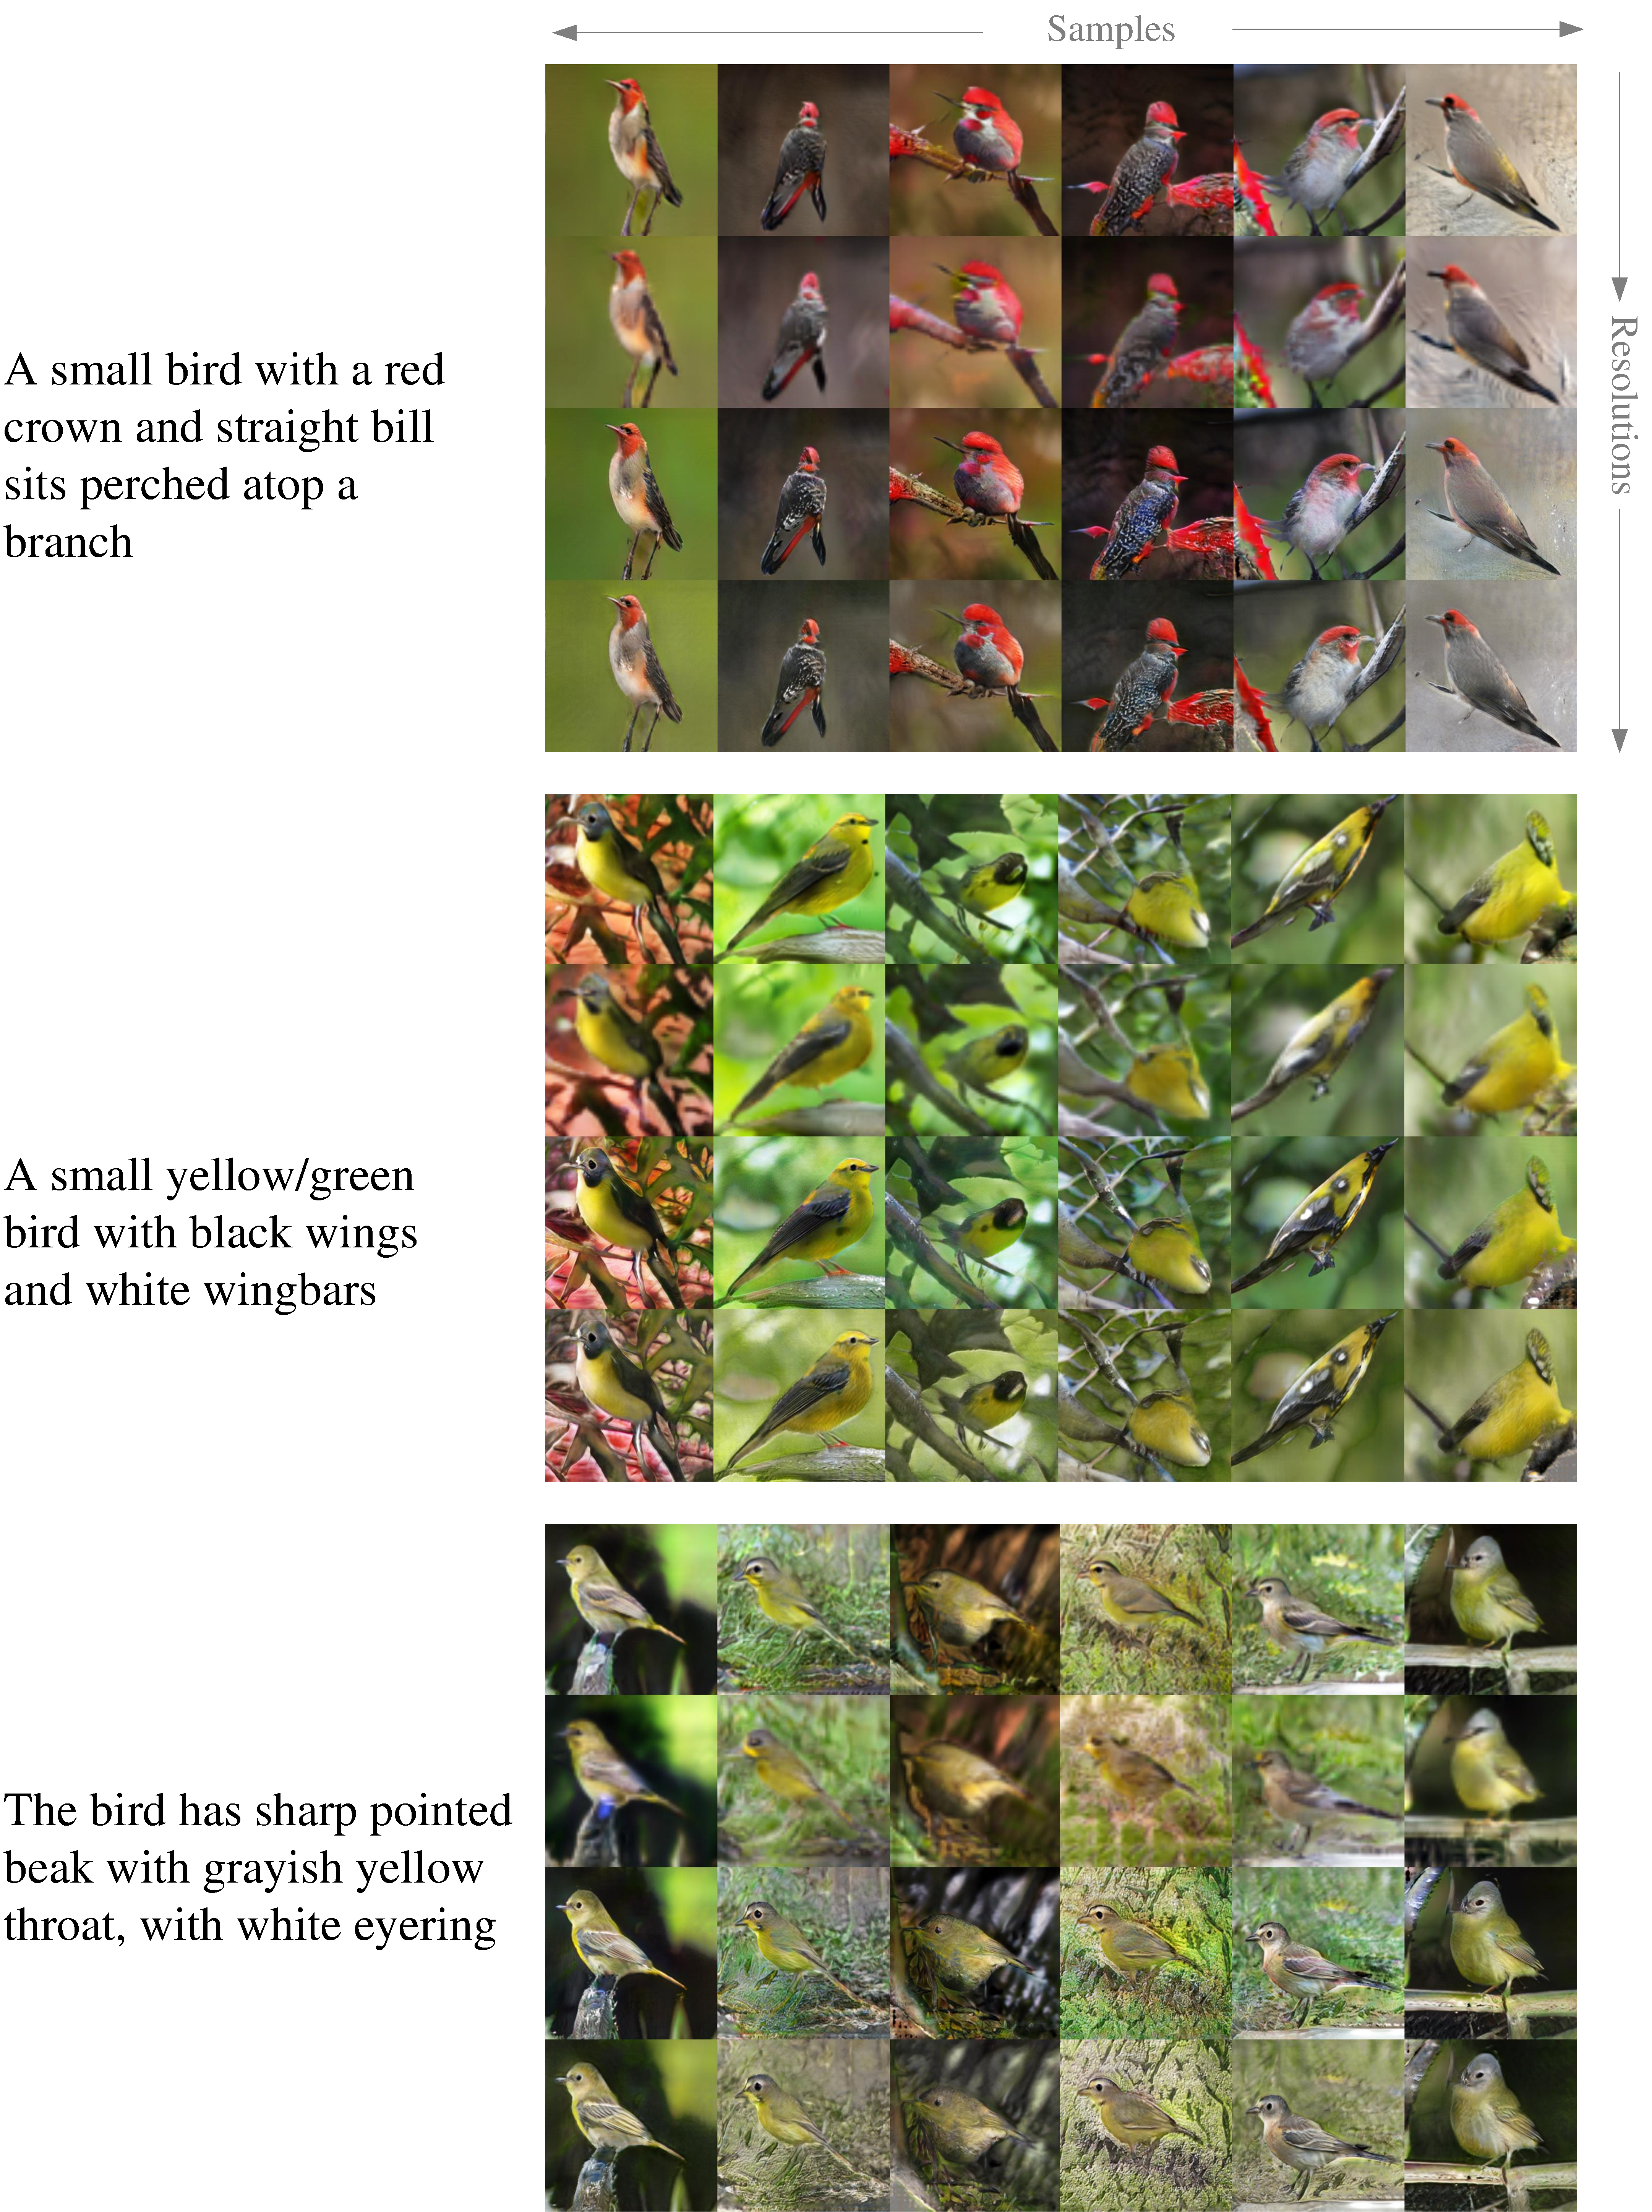
\includegraphics[width=0.9\textwidth]{figure/supp_bird.pdf}

	\caption{Sample results on CUB. For each input, 6 samples with resolutions of $64^2$, $128^2$, $256^2$, and $512^2$ are shown in 4 rows, respectively. }  
	\label{fig:bird}
\end{figure}

\newpage

%\subsection{Results on the Oxford-102 flower dataset}

\begin{figure}[th!]
	\centering
	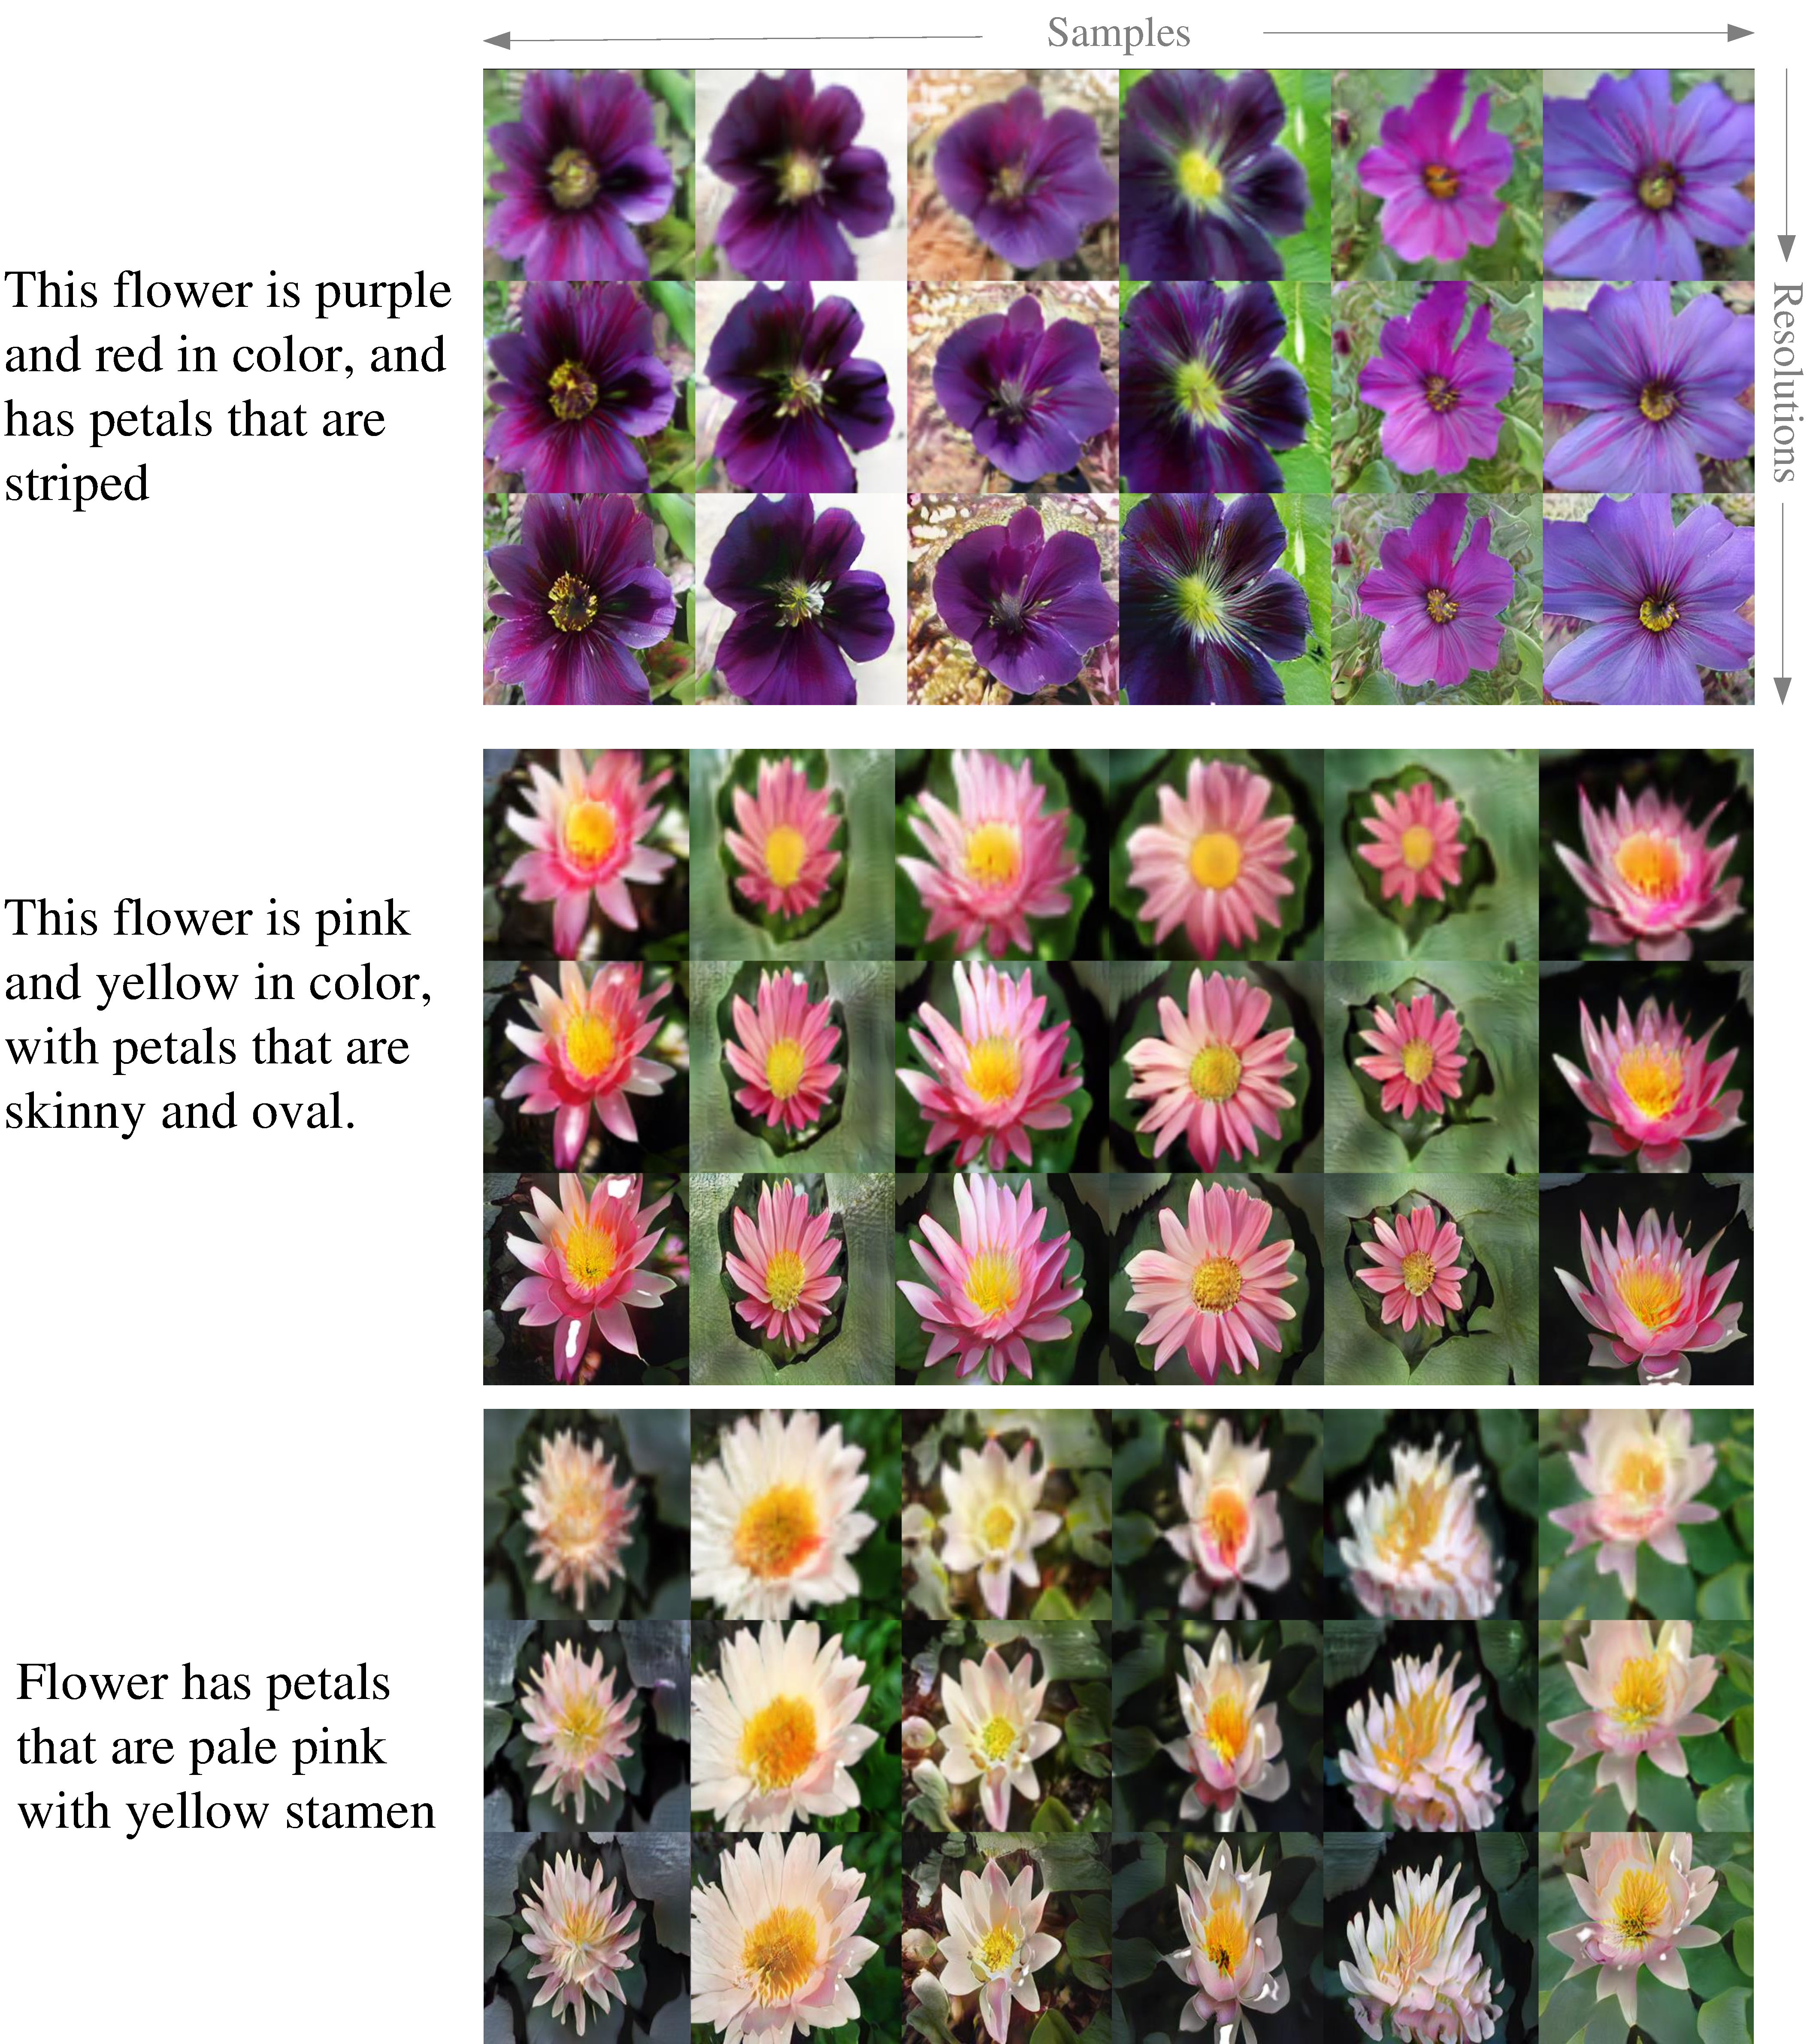
\includegraphics[width=0.999\textwidth]{figure/supp_flower.pdf}
	
	\caption{Sample results on Oxford-102. For each input,  6 samples with resolutions of $64^2$, $128^2$, and $256^2$ are shown in 3 rows, respectively. }  
	\label{fig:flower}
\end{figure}
%\subsection{More results on COCO}
\begin{figure}[ht!]
	\centering
	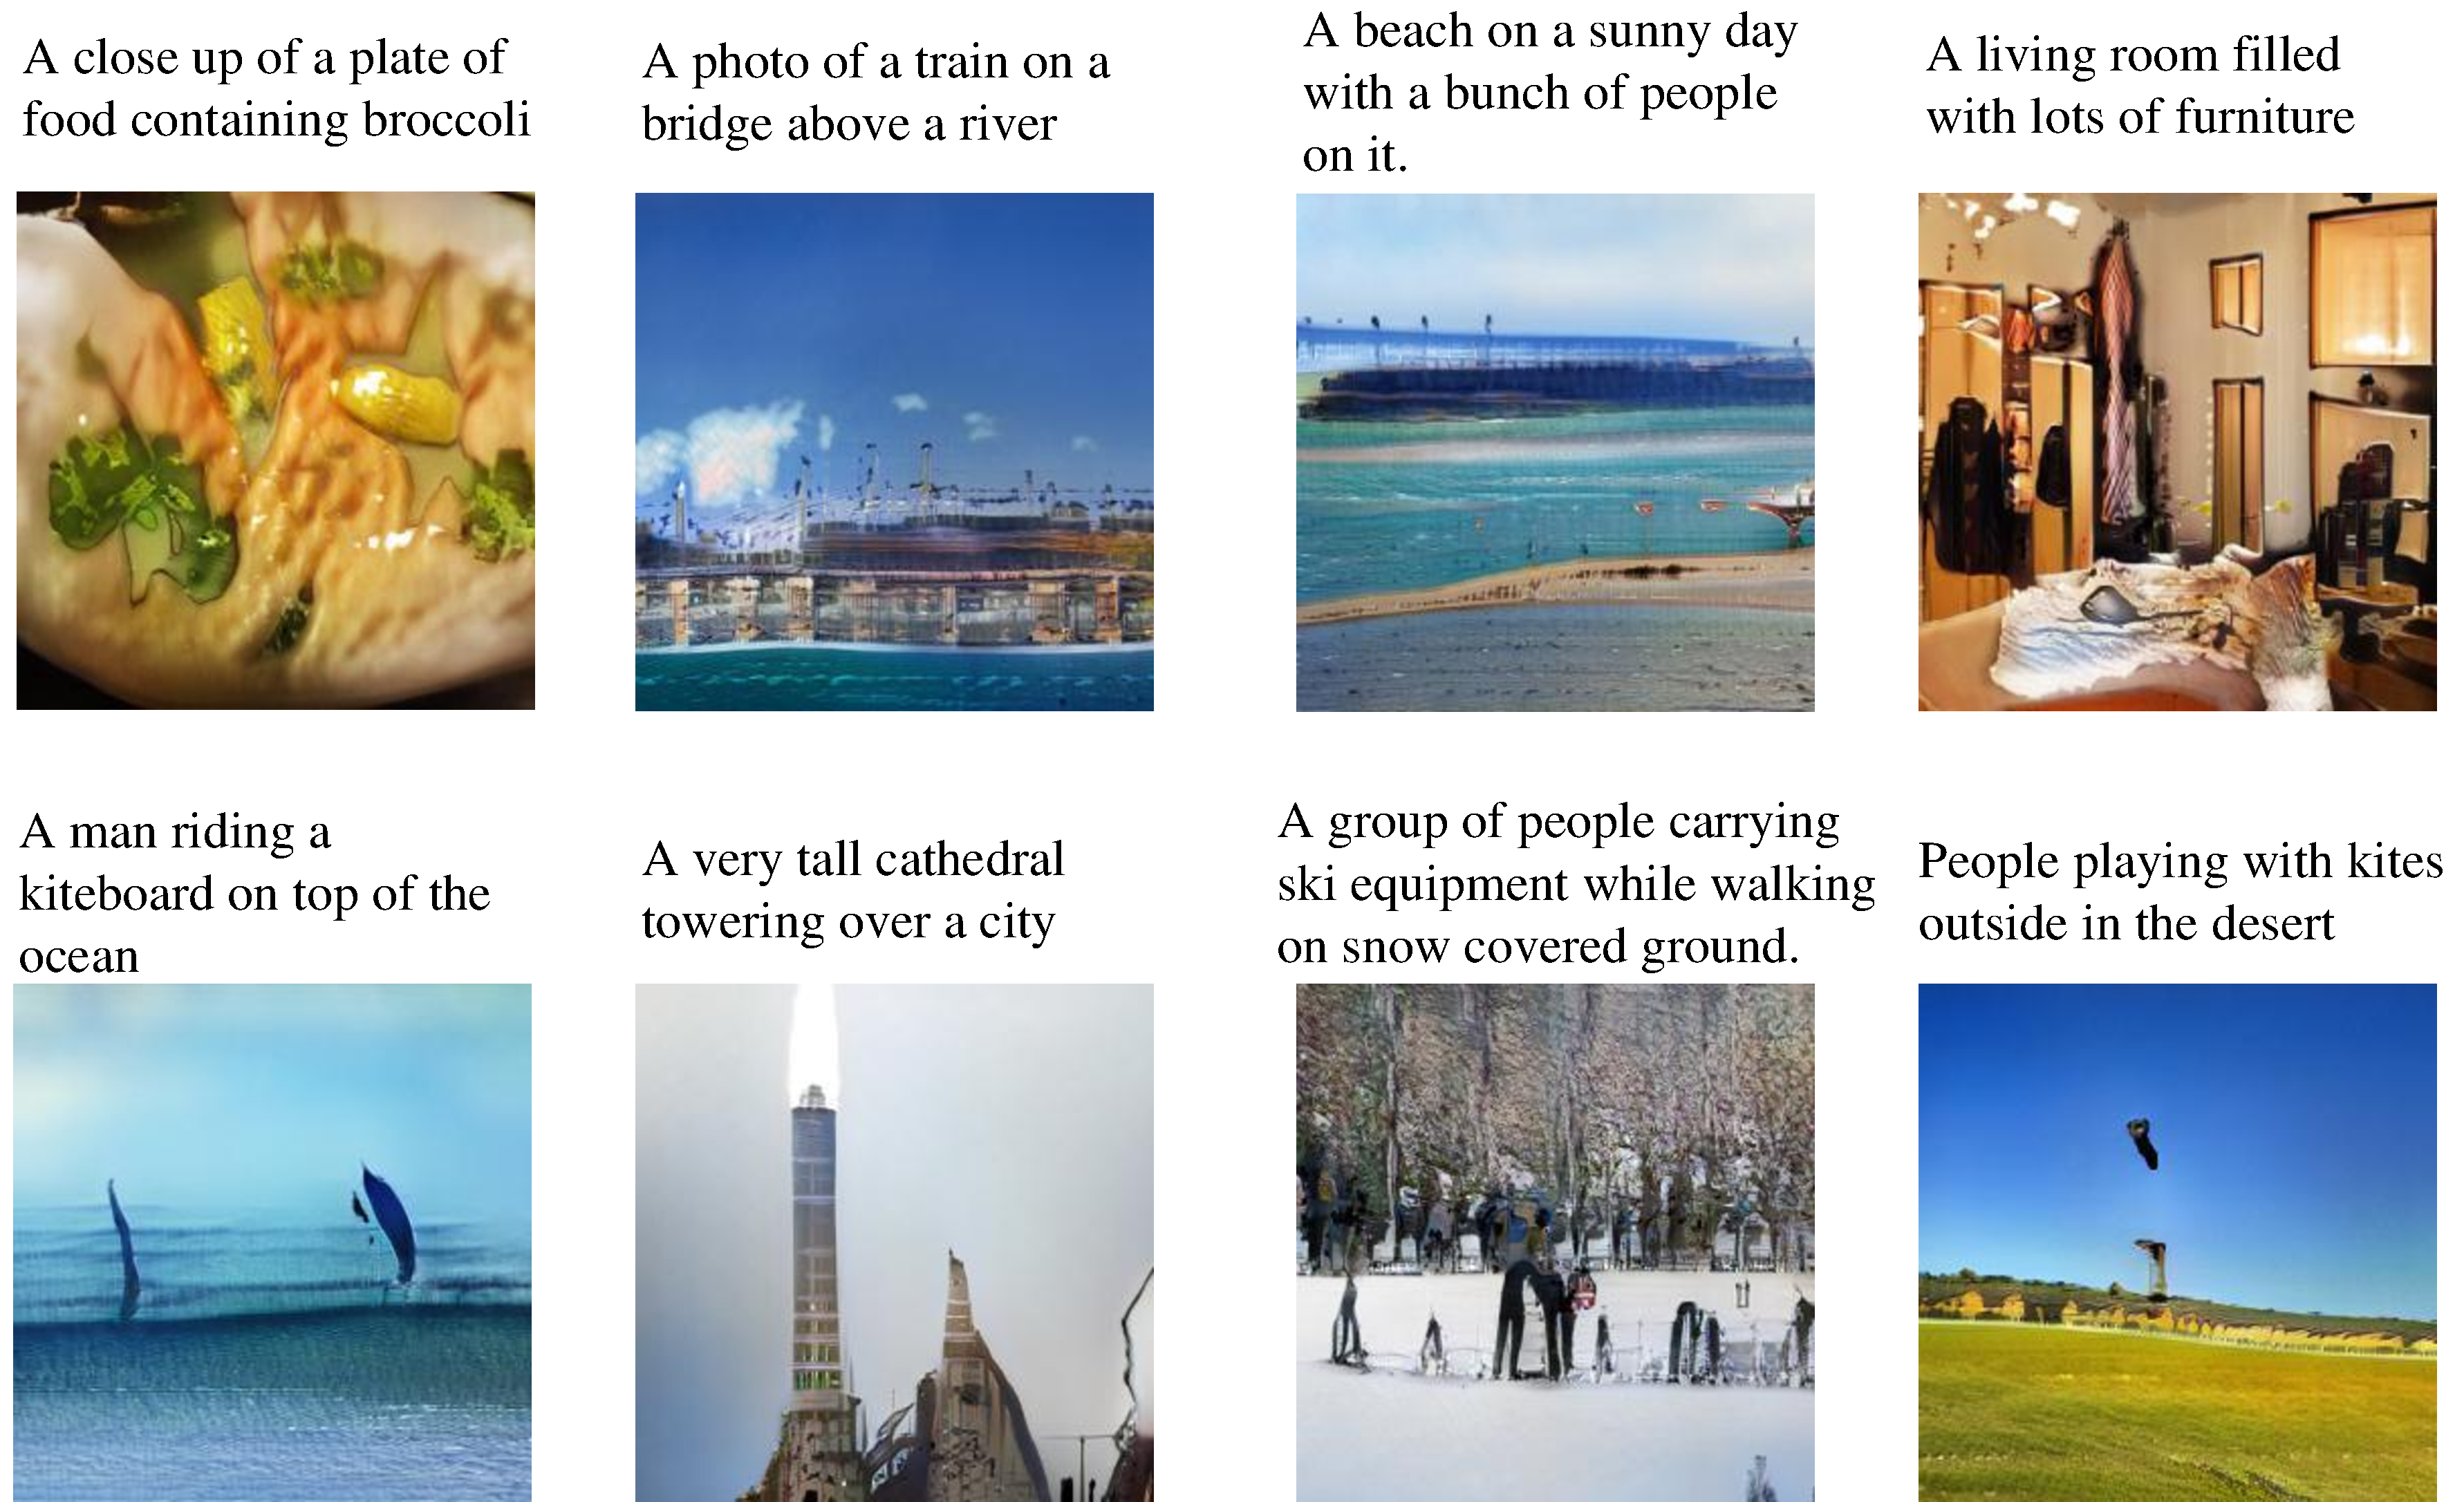
\includegraphics[width=0.8\textwidth,width=0.8\textwidth]{figure/supp_coco.pdf}
	
	\caption{Sample results on COCO. We show 8 $256^2$ samples in very different scenes. }  
	\label{fig:coco}
\end{figure}



{\small
	\bibliographystyle{ieee}
	\bibliography{reference_zizhao,egbib}
}

\end{document}
